\documentclass[11pt,a4paper]{article}

% ── Idioma y codificacion ─────────────────────────────────────────────
\usepackage[utf8]{inputenc}
\usepackage[T1]{fontenc}
\usepackage[spanish]{babel}

% ── Layout y tipografia ──────────────────────────────────────────────
\usepackage[margin=2.5cm]{geometry}
\usepackage{microtype}
\usepackage{parskip}
\usepackage{setspace}
\onehalfspacing

% ── Tablas y figuras ─────────────────────────────────────────────────
\usepackage{booktabs}
\usepackage{tabularx}
\usepackage{longtable}
\usepackage{multirow}
\usepackage[table]{xcolor}
\usepackage{colortbl}
\usepackage{graphicx}
\usepackage{float}

% ── Listas compactas ─────────────────────────────────────────────────
\usepackage{enumitem}
\setlist[itemize]{nosep, leftmargin=*, topsep=2pt, partopsep=0pt}
\setlist[enumerate]{nosep, leftmargin=*, topsep=2pt, partopsep=0pt}

% ── Cajas y destacados ──────────────────────────────────────────────
\usepackage[most]{tcolorbox}

% ── Headers y footers ────────────────────────────────────────────────
\usepackage{fancyhdr}
\pagestyle{fancy}
\fancyhf{}
\fancyhead[L]{\small Introducci\'{o}n a la Ciencia de Datos 2026}
\fancyhead[R]{\small Tarea 2}
\fancyfoot[C]{\thepage}
\renewcommand{\headrulewidth}{0.4pt}

% ── Links ────────────────────────────────────────────────────────────
\usepackage[colorlinks=true, linkcolor=blue!70!black, urlcolor=blue!70!black, citecolor=blue!70!black]{hyperref}

% ── Penalizaciones para viudas y huerfanas ───────────────────────────
\widowpenalty=10000
\clubpenalty=10000

% ── Colores personalizados ───────────────────────────────────────────
\definecolor{udelar}{RGB}{0, 75, 135}
\definecolor{lightgray}{RGB}{245, 245, 245}
\definecolor{codebg}{RGB}{248, 248, 248}

% ── Codigo monoespaciado ─────────────────────────────────────────────
\usepackage{listings}
\lstset{
    basicstyle=\ttfamily\footnotesize,
    backgroundcolor=\color{codebg},
    frame=single,
    framerule=0pt,
    breaklines=true,
    breakatwhitespace=true,
    columns=fullflexible,
    keepspaces=true,
    xleftmargin=8pt,
    xrightmargin=8pt,
}

% ══════════════════════════════════════════════════════════════════════
\begin{document}

% ── CARATULA ─────────────────────────────────────────────────────────
\begin{titlepage}
\centering
\vspace*{1cm}


\includegraphics[width=0.8\textwidth]{Logo_Fing+Udelar_horizontal_RGB.png}\\
\vspace{1cm}

{\Huge\bfseries Tarea 2 \par}
\vspace{0.5cm}
{\Large\bfseries Introducci\'{o}n a la Ciencia de Datos \par}
\vspace{0.5cm}
{\Large\bfseries Edici\'{o}n 2026 \par}

\vfill

\begin{flushleft}
\large
\textbf{Integrantes:}
\vspace{0.3cm}
\begin{itemize}[label={}, left=0pt]
    \item Tom\'{a}s Alejo Spoturno Gonzalez, 5.165.789-6
    \item Nicol\'{a}s Buero, 5.000.105-4
\end{itemize}
\end{flushleft}

\vfill

\textbf{Universidad de la Rep\'{u}blica}\\
\textbf{Facultad de Ingenier\'{\i}a}\\
\vspace{1cm}
Junio 2026

\end{titlepage}

% ── INDICE ───────────────────────────────────────────────────────────
\newpage
\tableofcontents
\newpage

% ══════════════════════════════════════════════════════════════════════
% INTRODUCCION
% ══════════════════════════════════════════════════════════════════════
\section{Introducci\'{o}n}

Este informe documenta la resoluci\'{o}n de la Tarea~2 del curso \textit{Introducci\'{o}n a la Ciencia de Datos} (edici\'{o}n 2026). La tarea es continuaci\'{o}n directa de la Tarea~1 y utiliza el mismo dataset: un subconjunto muestreado del corpus abierto \textit{All the News 2.1 -- Component One}, que contiene art\'{\i}culos de noticias publicados en distintos medios de prensa. El objetivo de esta entrega es \textbf{construir y evaluar clasificadores autom\'{a}ticos de texto} que identifiquen a qu\'{e} medio pertenece cada art\'{\i}culo, partiendo de representaciones num\'{e}ricas del texto.

El trabajo se estructura en dos partes. La Parte~1 cubre la preparaci\'{o}n de los datos, la representaci\'{o}n num\'{e}rica del texto mediante \textit{Bag of Words} y TF-IDF, y una exploraci\'{o}n visual con PCA. La Parte~2 cubre el entrenamiento, la validaci\'{o}n y la comparaci\'{o}n de modelos de clasificaci\'{o}n.

El c\'{o}digo que genera los resultados est\'{a} en el notebook \texttt{Tarea\_2/2026\_tarea2.ipynb} del repositorio p\'{u}blico \url{https://github.com/Nicolasvb23/intro-cd}.

% ══════════════════════════════════════════════════════════════════════
% PARTE 1
% ══════════════════════════════════════════════════════════════════════
\section{Parte 1: Dataset y representaci\'{o}n num\'{e}rica de texto}

\subsection{Preparaci\'{o}n del dataset}

El proceso de limpieza de datos y la funci\'{o}n \texttt{clean\_text} son los mismos que en la Tarea~1, a los que se remite para el detalle. En resumen, sobre el dataset original de 30.213 art\'{\i}culos se eliminaron 141 filas con \texttt{publication} nula, 1.176 con \texttt{article} nulo o placeholder, y 13 duplicados exactos, resultando en \textbf{29.024 art\'{\i}culos limpios}. La funci\'{o}n \texttt{clean\_text} aplica los mismos pasos que en la entrega anterior (eliminaci\'{o}n de cabecera, minusc\'{u}las, URLs, puntuaci\'{o}n, n\'{u}meros aislados y normalizaci\'{o}n de espacios), sin agregar filtrado de \textit{stopwords} ni identificadores de medios en esta etapa, ya que esas decisiones se toman a nivel del vectorizador y son parte del an\'{a}lisis de la Secci\'{o}n~\ref{sec:pca}.

\subsubsection*{Selecci\'{o}n de los tres medios principales}

El an\'{a}lisis de esta tarea se restringe a los \textbf{tres medios con mayor cantidad de art\'{\i}culos} en \texttt{df\_clean}. Los recuentos se muestran en la Tabla~\ref{tab:top3}.

\begin{table}[H]
\centering
\caption{Top~3 medios de prensa por cantidad de art\'iculos en el dataset limpio.}
\label{tab:top3}
\begin{tabular}{l r r}
\toprule
\textbf{Medio} & \textbf{Art\'iculos} & \textbf{\% del total (top~3)} \\
\midrule
Reuters & 9.266 & 63,2\% \\
The New York Times & 2.805 & 19,1\% \\
CNBC & 2.578 & 17,6\% \\
\midrule
\textbf{Total top~3} & \textbf{14.649} & \textbf{100\%} \\
\bottomrule
\end{tabular}
\end{table}

Los tres medios coinciden con los tres primeros del top~5 de la Tarea~1. El dataset resultante presenta un \textbf{desbalance pronunciado}: \textit{Reuters} acumula el 63,2\% de los art\'{\i}culos, frente al 19,1\% de \textit{NYT} y el 17,6\% de \textit{CNBC}. Esto tiene implicancias sobre las m\'{e}tricas de evaluaci\'{o}n que se discuten en la Parte~2.

\subsubsection*{Partici\'{o}n train/test}

El dataset de los tres medios se dividi\'{o} en un conjunto de \textbf{entrenamiento (70\%)} y un conjunto de \textbf{test (30\%)}, utilizando muestreo estratificado por medio de prensa (\texttt{stratify=y}). La estratificaci\'{o}n garantiza que la proporci\'{o}n de art\'{\i}culos de cada medio sea la misma en ambos conjuntos. Se fij\'{o} \texttt{random\_state=23} para reproducibilidad.

\subsection{Verificaci\'{o}n del balance de clases}

\begin{figure}[H]
\centering
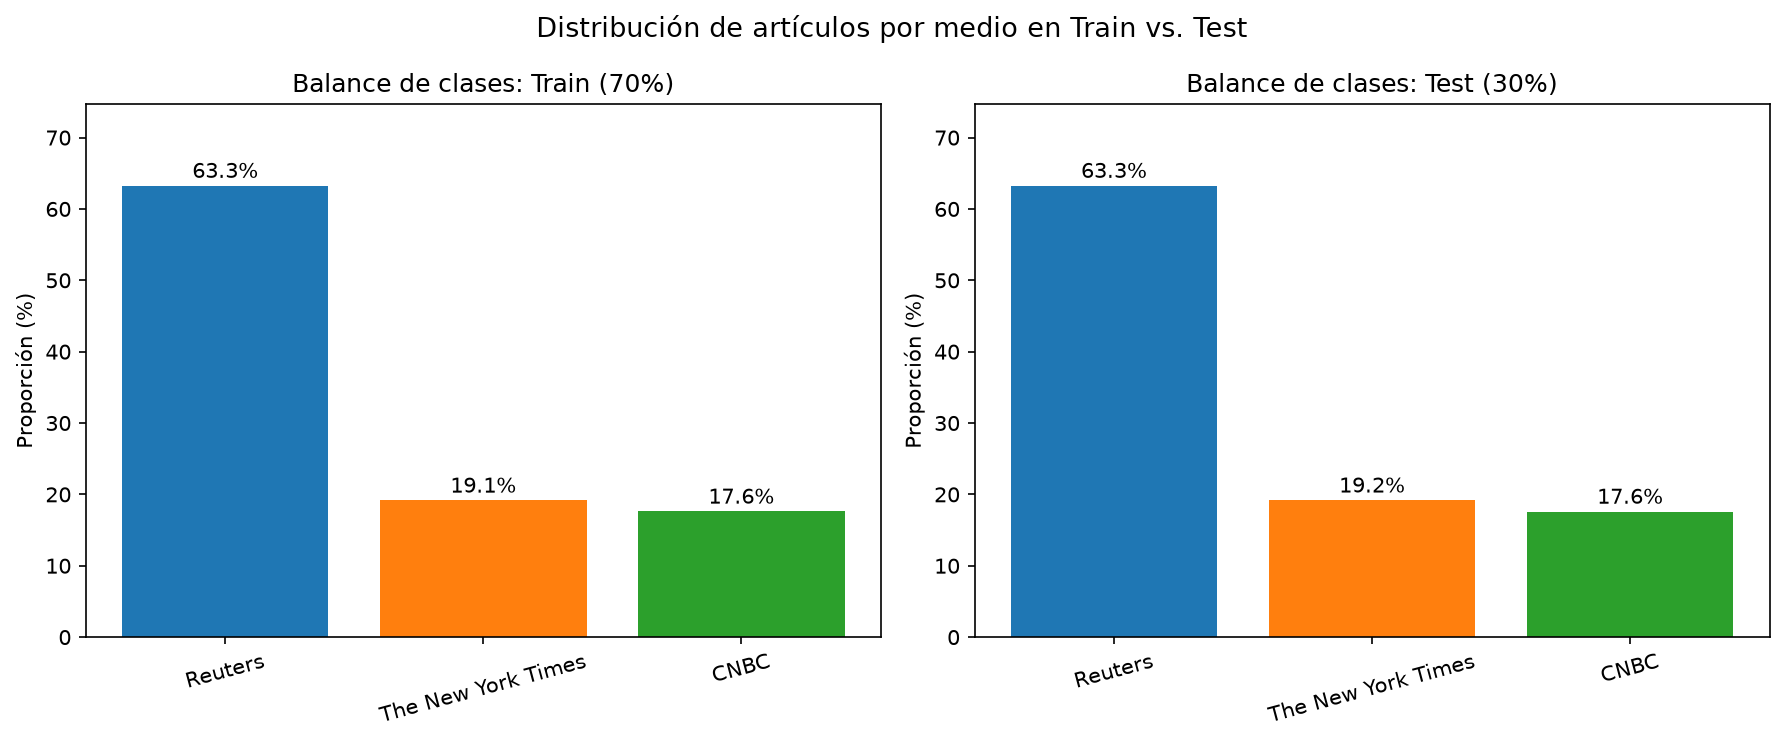
\includegraphics[width=0.95\textwidth]{imagenes/chart_balance.png}
\caption{Proporci\'{o}n de art\'iculos de cada medio en los conjuntos de entrenamiento (izquierda) y test (derecha). La estratificaci\'{o}n garantiza distribuciones id\'{e}nticas en ambos conjuntos.}
\label{fig:balance}
\end{figure}

La Figura~\ref{fig:balance} confirma que las proporciones son id\'{e}nticas en train y test, como se espera de un split estratificado. El desbalance del dataset se preserva de forma exacta: aproximadamente 62\% de los art\'{\i}culos corresponden a \textit{Reuters}, lo que implica que un clasificador trivial que siempre prediga ``Reuters'' alcanzar\'{\i}a un \textit{accuracy} de ese orden sin aprender nada del contenido. Este punto se retoma en la Parte~2 al discutir las limitaciones del \textit{accuracy} como \'{u}nica m\'{e}trica.

\subsection{Representaci\'{o}n Bag of Words}

\subsubsection*{C\'{o}mo funciona}

La representaci\'{o}n \textit{Bag of Words} (BoW) convierte cada documento en un vector num\'{e}rico de la siguiente manera: se construye un \textbf{vocabulario} fijo con todas las palabras distintas que aparecen en el corpus de entrenamiento, y cada documento se representa como un vector de tama\~{n}o igual al vocabulario donde la posici\'{o}n $j$ contiene la \textbf{cantidad de veces} que la palabra $j$ aparece en ese documento. El orden de las palabras dentro del texto se ignora completamente.

\subsubsection*{Tama\~{n}o de la matriz}

Se ajust\'{o} un \texttt{CountVectorizer} con par\'{a}metros por defecto sobre el conjunto de entrenamiento. La matriz resultante tiene dimensiones $[\text{n\_docs} \times \text{n\_palabras}]$, donde:
\begin{itemize}
    \item \textbf{Filas}: la cantidad de art\'{\i}culos en el conjunto de entrenamiento ([TODO] art\'{\i}culos).
    \item \textbf{Columnas}: el tama\~{n}o del vocabulario aprendido sobre el train ([TODO] palabras distintas).
\end{itemize}

\subsubsection*{Por qu\'{e} es una matriz \textit{sparse}}

Si se almacenara como una matriz densa (todos los valores en memoria), la matriz BoW ocupar\'{\i}a aproximadamente:
\[
[\text{TODO}] \times [\text{TODO}] \times 8\ \text{bytes} \approx [\text{TODO}]\ \text{MB}
\]
Esto ser\'{\i}a inmanejable incluso con este dataset reducido. Sin embargo, la gran mayor\'{\i}a de las entradas son cero: la densidad de la matriz es del orden del 0,2\%---0,4\%, lo que significa que m\'{a}s del 99\% de sus valores son cero. Ninguna nota usa m\'{a}s de unos cientos de palabras distintas, mientras que el vocabulario total tiene decenas de miles. Las matrices \textit{sparse} almacenan \'{u}nicamente los valores no-nulos y sus posiciones (formato CSR), lo que reduce el uso de memoria en varios \'{o}rdenes de magnitud.

Si en lugar de 14.000 art\'{\i}culos tuvi\'{e}ramos el dataset completo de 1,8 millones de art\'{\i}culos del corpus original y un vocabulario de cientos de miles de palabras, la matriz densa ser\'{\i}a completamente inviable en cualquier equipo de c\'{o}mputo est\'{a}ndar.

\subsection{Representaci\'{o}n TF-IDF}

\subsubsection*{Qu\'{e} es un n-grama}

Un \textbf{n-grama} es una secuencia contigua de $n$ tokens (palabras o caracteres). Un unigrama ($n=1$) es una palabra individual; un bigrama ($n=2$) es un par de palabras consecutivas. Por ejemplo, a partir del texto \textit{``the new york times''} se extraen los bigramas \textit{``the new''}, \textit{``new york''} y \textit{``york times''}. Incluir bigramas en el vocabulario permite capturar expresiones compuestas y contexto local que los unigramas no pueden representar. El par\'{a}metro \texttt{ngram\_range=(1,2)} en el vectorizador combina unigramas y bigramas en el mismo vocabulario, aunque a costa de aumentar dram\'{a}ticamente el n\'{u}mero de columnas.

\subsubsection*{La transformaci\'{o}n TF-IDF}

El principal problema de BoW es que las palabras muy frecuentes en todo el corpus (art\'{\i}culos, preposiciones, conjunciones) dominan los vectores aunque no aporten informaci\'{o}n discriminante entre medios. TF-IDF (\textit{Term Frequency -- Inverse Document Frequency}) corrige esto ponderando cada conteo por la siguiente expresi\'{o}n:

\[
\text{TF-IDF}(t, d) = \text{TF}(t, d) \times \text{IDF}(t)
\]

donde $\text{TF}(t, d)$ es la frecuencia normalizada del t\'{e}rmino $t$ en el documento $d$, e $\text{IDF}(t) = \log\!\left(\frac{N+1}{n_t+1}\right) + 1$ con $N$ el n\'{u}mero total de documentos y $n_t$ la cantidad de documentos que contienen $t$. La transformaci\'{o}n tiene dos efectos:
\begin{itemize}
    \item \textbf{Penaliza t\'{e}rminos ubicuos}: una palabra que aparece en todos o casi todos los documentos tiene IDF $\approx 0$, por lo que su peso TF-IDF cae a cero o pr\'{o}ximo a cero, independientemente de cu\'{a}ntas veces aparezca en un documento dado.
    \item \textbf{Premia t\'{e}rminos discriminantes}: una palabra rara que aparece mucho en un documento particular y poco en el resto recibe un peso alto.
\end{itemize}

El vectorizador \texttt{TfidfVectorizer} se ajusta \'{u}nicamente sobre el conjunto de entrenamiento (\texttt{fit\_transform}). El vocabulario y los valores IDF aprendidos se aplican luego sobre el conjunto de test (\texttt{transform}), sin recalcular nada sobre el test. Esto simula correctamente el escenario real donde el modelo no tiene acceso a los datos de evaluaci\'{o}n al momento de entrenarse.

\subsection{Visualizaci\'{o}n PCA sobre TF-IDF}
\label{sec:pca}

\subsubsection*{Consideraciones de implementaci\'{o}n}

El an\'{a}lisis de componentes principales (\textit{PCA}) requiere materializar la matriz TF-IDF como densa para poder centrarla. Con el vocabulario completo de 85.152 palabras y 10.254 documentos de entrenamiento, esto supone aproximadamente 6,9~GB en RAM. En esta tarea se opt\'{o} por utilizar directamente \texttt{sklearn.decomposition.PCA}, materializando la matriz completa con \texttt{.toarray()}. Como alternativa sin restricciones de memoria, \texttt{TruncatedSVD} opera sobre la representaci\'{o}n \textit{sparse} sin densificarla, aunque sin centrar los datos previamente.

\subsubsection*{Resultados con la configuraci\'{o}n base}

\begin{figure}[H]
\centering
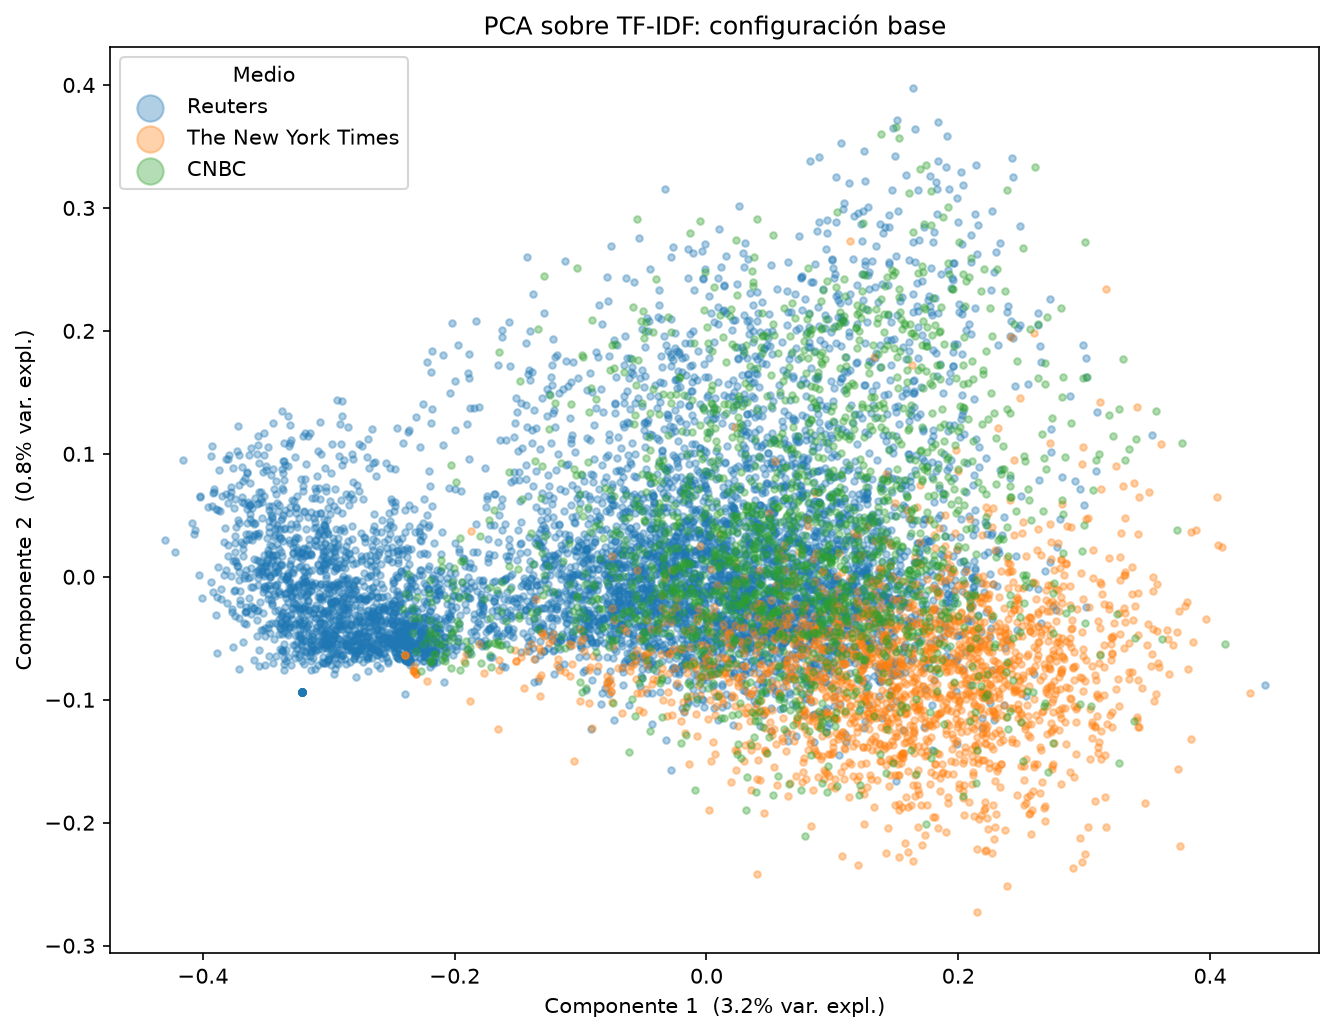
\includegraphics[width=0.85\textwidth]{imagenes/chart_pca_base.png}
\caption{Mapa PCA (2 primeras componentes) sobre TF-IDF base, coloreado por medio de prensa.}
\label{fig:pca_base}
\end{figure}

La Figura~\ref{fig:pca_base} muestra el conjunto de entrenamiento proyectado sobre las dos primeras componentes principales. Se observa que \textit{Reuters} forma una nube claramente separada del resto, especialmente a lo largo de la primera componente. Esto es esperable dado que \textit{Reuters} tiene pistas l\'{e}xicas muy marcadas que se discuten m\'{a}s adelante. \textit{NYT} y \textit{CNBC} presentan mayor superposici\'{o}n entre s\'{\i}, aunque con cierta separaci\'{o}n.

Las dos primeras componentes explican solo [TODO]\% de la varianza total, lo que indica que \textbf{no es posible separar los tres medios de forma perfecta con \'{u}nicamente 2 componentes}. Los vectores TF-IDF viven en un espacio de alta dimensionalidad y la proyecci\'{o}n bidimensional pierde la mayor\'{\i}a de la informaci\'{o}n.

\subsubsection*{Comparaci\'{o}n de configuraciones}

\begin{figure}[H]
\centering
\includegraphics[width=\textwidth]{imagenes/chart_pca_configs.png}
\caption{PCA con cuatro configuraciones distintas del \texttt{TfidfVectorizer}: base, con \textit{stop words}, sin IDF y con bigramas.}
\label{fig:pca_configs}
\end{figure}

La Figura~\ref{fig:pca_configs} compara las cuatro configuraciones pedidas. Las observaciones principales son:

\paragraph{a) Filtrado de \textit{stop words} (\texttt{stop\_words='english'}).}
Al eliminar las palabras funcionales del ingl\'{e}s (art\'{\i}culos, preposiciones, conjunciones), el vocabulario se reduce y los vectores quedan dominados por t\'{e}rminos de contenido. La separaci\'{o}n entre medios tiende a mejorar levemente porque se eliminan dimensiones que son equidistribuidas entre todos los documentos y no aportan discriminaci\'{o}n. La varianza explicada por las primeras dos componentes suele aumentar respecto a la configuraci\'{o}n base.

\paragraph{b) Sin IDF (\texttt{use\_idf=False}).}
Con IDF desactivado, los vectores contienen directamente la frecuencia relativa del t\'{e}rmino en el documento (TF puro). Las palabras muy comunes recuperan el peso que IDF les quitaba. La separaci\'{o}n entre medios se deteriora notablemente porque los t\'{e}rminos ubicuos vuelven a dominar las componentes principales, reduciendo la varianza explicada en las primeras componentes y comprimiendo los puntos en un espacio m\'{a}s denso y menos separable.

\paragraph{c) Bigramas (\texttt{ngram\_range=(1,2)}).}
Al agregar bigramas el vocabulario se expande varios veces (incluye ahora todas las secuencias de dos palabras consecutivas). Los vectores resultantes capturan m\'{a}s contexto local. La separaci\'{o}n en el PCA puede mejorar o mantenerse similar a la base, pero el costo computacional aumenta considerablemente. Patrones como \textit{``reuters reporting''} o \textit{``new york''} pasan a ser features expl\'{\i}citas.

\subsubsection*{Varianza explicada}

\begin{figure}[H]
\centering
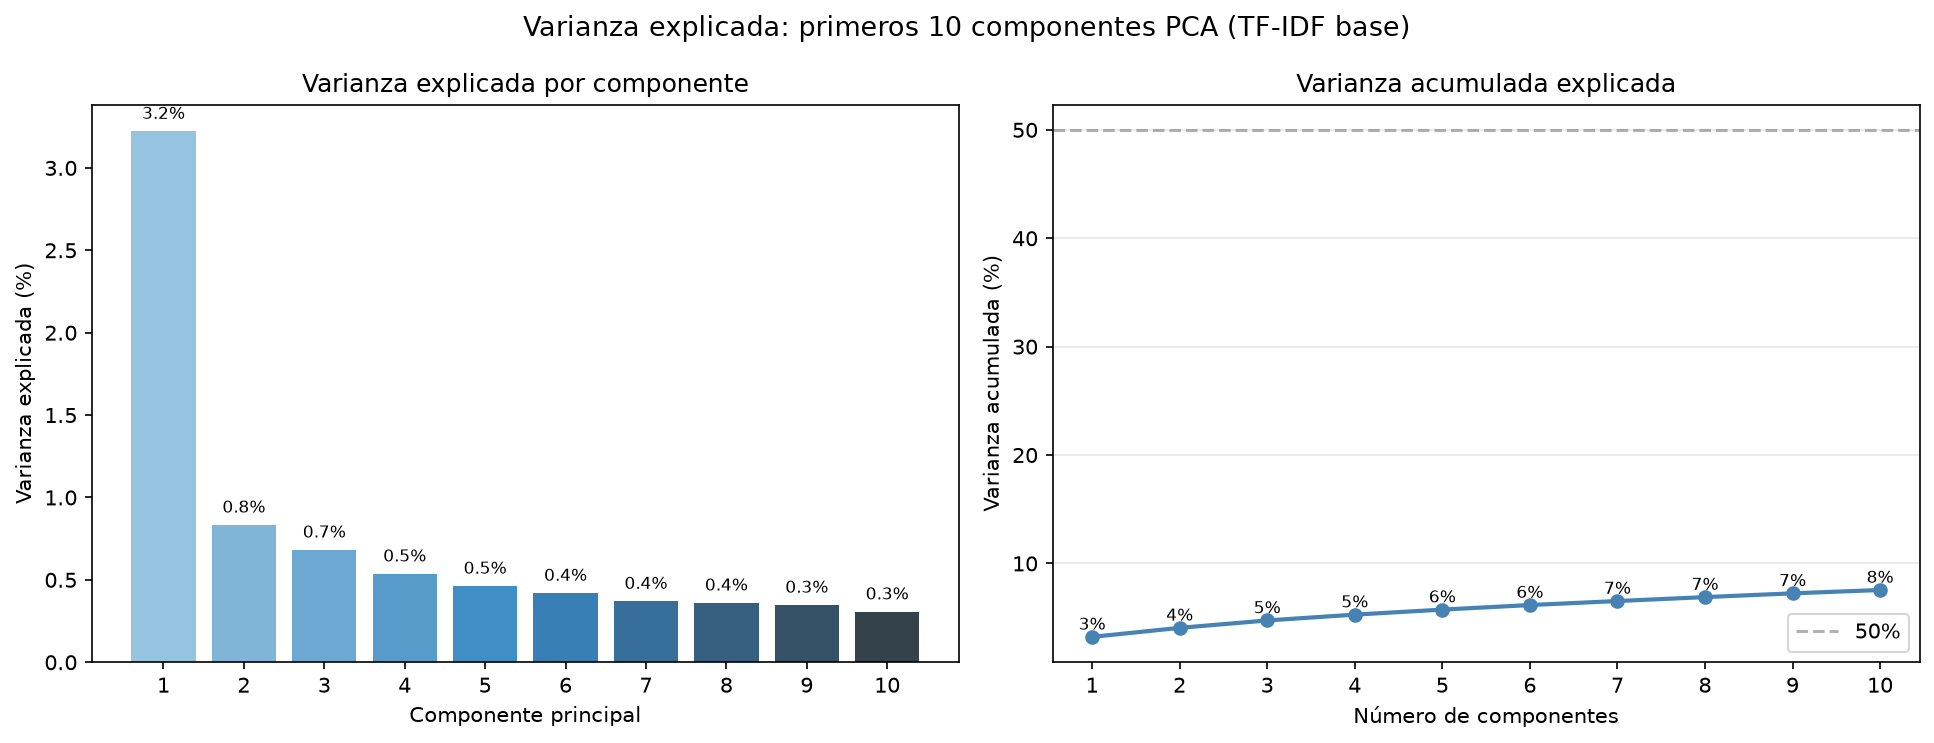
\includegraphics[width=\textwidth]{imagenes/chart_pca_variance.png}
\caption{Varianza explicada por cada componente principal (izquierda) y varianza acumulada (derecha) para los primeros 10 componentes sobre la configuraci\'{o}n TF-IDF base.}
\label{fig:pca_variance}
\end{figure}

La Figura~\ref{fig:pca_variance} muestra que la varianza explicada decrece r\'{a}pidamente con el n\'{u}mero de componentes y que incluso con 10 componentes la varianza acumulada es relativamente baja. Esto refleja la \textbf{alta dimensionalidad intr\'{\i}nseca del texto}: la informaci\'{o}n est\'{a} repartida entre miles de t\'{e}rminos, y ninguna direcci\'{o}n captura una fracci\'{o}n grande de la varianza total.

\subsubsection*{Origen de la separaci\'{o}n observada}

La separaci\'{o}n en el PCA puede deberse a tres fuentes distintas, que no son mutuamente excluyentes:

\begin{itemize}
    \item \textbf{Pistas expl\'{\i}citas del medio}: como se document\'{o} en la Tarea~1, \textit{Reuters} tiene el dateline \texttt{(Reuters)} en el 92\% de sus art\'{\i}culos, y \textit{The Hill} ten\'{\i}a el footer \texttt{Capitol Hill Publishing Corp.} en el 99\%. Aunque en esta tarea \textit{The Hill} ya no est\'{a} presente en el top~3, \textit{Reuters} sigue teniendo estas marcas, lo que crea un eje claro de separaci\'{o}n en las primeras componentes. Con la configuraci\'{o}n base (sin remoci\'{o}n de boilerplate), la separaci\'{o}n de \textit{Reuters} est\'{a} en gran medida impulsada por estos patrones.

    \item \textbf{Diferencias tem\'{a}ticas}: los tres medios cubren agendas distintas. \textit{Reuters} es una agencia de noticias generalista con fuerte cobertura financiera y de mercados; \textit{CNBC} se especializa en econom\'{\i}a y negocios; \textit{NYT} tiene una cobertura amplia que incluye pol\'{\i}tica, cultura y opini\'{o}n. Estas diferencias de cobertura generan vocabularios caracter\'{\i}sticos que contribuyen a la separaci\'{o}n incluso despu\'{e}s de remover las pistas directas.

    \item \textbf{Diferencias de estilo editorial}: independientemente del tema, cada medio tiene convenciones propias de escritura (largo de las notas, uso de citas, estructura de los p\'{a}rrafos, vocabulario t\'{e}cnico). Estas diferencias son m\'{a}s sutiles y podr\'{\i}an quedar capturadas en componentes de orden superior, no necesariamente en las primeras dos.
\end{itemize}

En la configuraci\'{o}n base, la primera componente est\'{a} muy probablemente dominada por las pistas expl\'{\i}citas de \textit{Reuters}. El filtrado de \textit{stop words} no elimina esas pistas; s\'{\i} lo har\'{\i}a remover el boilerplate mediante regex (como se hizo en la Parte~2 de la Tarea~1), pero ese procesamiento no es parte del an\'{a}lisis de esta secci\'{o}n.

\end{document}
